\chapter{Software Design Description}

\section{System Design \& Architecture}

\subsection{System Architecture Overview}
The **AR-IMMS** platform utilizes a modern microservice-ready modular architecture connecting edge collector agents, a high-throughput backend API, a real-time event streaming gateway, a web command center, and a mobile AR application.

\begin{figure}[H]
    \centering
    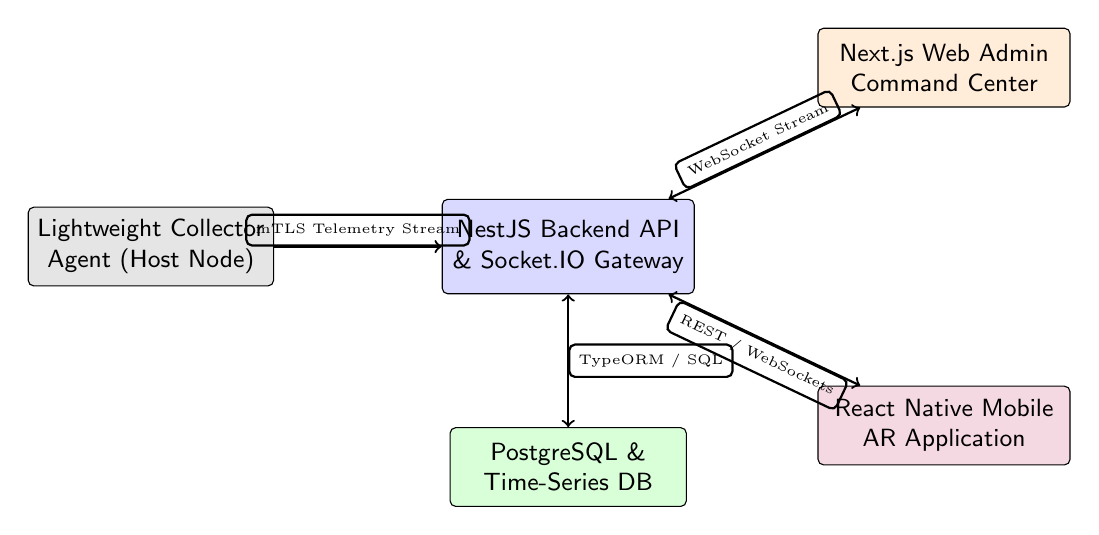
\begin{tikzpicture}[node distance=1.8cm, every node/.style={draw, rectangle, align=center, rounded corners=2pt, font=\sffamily\small}]
        % Nodes
        \node (agent) [fill=gray!20, minimum width=3cm, minimum height=1cm] {Lightweight Collector\\Agent (Host Node)};
        \node (backend) [right of=agent, xshift=3.5cm, fill=blue!15, minimum width=3.2cm, minimum height=1.2cm] {NestJS Backend API\\\& Socket.IO Gateway};
        \node (db) [below of=backend, yshift=-1cm, fill=green!15, minimum width=3cm, minimum height=1cm] {PostgreSQL \&\\Time-Series DB};
        \node (web) [above right of=backend, xshift=3.5cm, yshift=1cm, fill=orange!15, minimum width=3.2cm, minimum height=1cm] {Next.js Web Admin\\Command Center};
        \node (ar) [below right of=backend, xshift=3.5cm, yshift=-1cm, fill=purple!15, minimum width=3.2cm, minimum height=1cm] {React Native Mobile\\AR Application};
        
        % Connectors
        \draw [->, thick] (agent) -- node[above, font=\tiny] {mTLS Telemetry Stream} (backend);
        \draw [<->, thick] (backend) -- node[right, font=\tiny] {TypeORM / SQL} (db);
        \draw [<->, thick] (backend) -- node[above, sloped, font=\tiny] {WebSocket Stream} (web);
        \draw [<->, thick] (backend) -- node[below, sloped, font=\tiny] {REST / WebSockets} (ar);
    \end{tikzpicture}
    \caption{AR-IMMS High-Level System Architecture}
\end{figure}

\section{Database Design}

\subsection{Entity-Relationship Overview}
The relational schema manages system metadata, spatial infrastructure hierarchy, time-series telemetry logs, alerting rules, and ticket workflows.

\begin{table}[H]
    \centering
    \caption{Core Database Tables Overview}
    \begin{tabular}{|l|p{11cm}|}
        \hline
        \textbf{Table Name} & \textbf{Description \& Primary Keys} \\ \hline
        \texttt{users} & Stores account credentials, full names, emails, and active status. (PK: \texttt{id}) \\ \hline
        \texttt{roles} & System RBAC roles (Admin, Operator, Technician). (PK: \texttt{id}) \\ \hline
        \texttt{sites} & Physical facility data center sites. (PK: \texttt{id}) \\ \hline
        \texttt{rooms} & Server rooms within data center sites. (PK: \texttt{id}, FK: \texttt{site\_id}) \\ \hline
        \texttt{racks} & Server racks located in specific rooms. (PK: \texttt{id}, FK: \texttt{room\_id}) \\ \hline
        \texttt{nodes} & Physical server nodes housed in racks. (PK: \texttt{id}, FK: \texttt{rack\_id}, \texttt{marker\_id}) \\ \hline
        \texttt{containers} & Docker container workloads running on nodes. (PK: \texttt{id}, FK: \texttt{node\_id}) \\ \hline
        \texttt{aruco\_markers} & Spatial QR/ArUco marker identifier dictionary. (PK: \texttt{id}) \\ \hline
        \texttt{telemetry\_logs} & High-frequency time-series metrics (CPU, RAM, Temp). (PK: \texttt{id}, FK: \texttt{node\_id}) \\ \hline
        \texttt{alerts} & Threshold breach and heartbeat timeout events. (PK: \texttt{id}, FK: \texttt{node\_id}) \\ \hline
        \texttt{tickets} & Maintenance tickets assigned to technicians. (PK: \texttt{id}, FK: \texttt{alert\_id}, \texttt{technician\_id}) \\ \hline
        \texttt{audit\_logs} & Immutable activity and security audit records. (PK: \texttt{id}, FK: \texttt{user\_id}) \\ \hline
    \end{tabular}
\end{table}

\section{Detailed Design}

\subsection{Class Diagram: Core Domain Models}
\begin{table}[H]
    \centering
    \caption{Domain Model Class Specifications}
    \begin{tabular}{|l|l|p{7cm}|}
        \hline
        \textbf{Class Name} & \textbf{Attributes} & \textbf{Key Methods} \\ \hline
        \texttt{ServerNode} & \texttt{id, name, ipAddress, status, rackId} & \texttt{getTelemetry(), updateStatus(), linkMarker()} \\ \hline
        \texttt{TelemetryAgent} & \texttt{agentId, nodeGuid, interval, certs} & \texttt{collectMetrics(), streamWebSocket(), retryBuffer()} \\ \hline
        \texttt{ARController} & \texttt{cameraFeed, markerId, trackedMatrix} & \texttt{detectMarker(), renderHUD(), fetchNodeMetrics()} \\ \hline
        \texttt{TicketEngine} & \texttt{ticketId, alertRef, status, assignedTo} & \texttt{assignTechnician(), logAction(), verifyClosure()} \\ \hline
    \end{tabular}
\end{table}

\subsection{Sequence Diagram: Real-Time Telemetry \& AR Camera Overlay}
The sequence below illustrates the flow from edge metric collection to mobile AR camera overlay display:

\begin{enumerate}
    \item \textbf{Collector Agent} captures hardware metrics (CPU, RAM, Docker stats) from the host machine every 5 seconds.
    \item Agent transmits encrypted metric payload over mTLS to the \textbf{NestJS Backend Gateway}.
    \item Backend persists metrics to \textbf{Time-Series DB} and broadcasts event payload over \textbf{Socket.IO} to connected Web and Mobile clients.
    \item On-site technician points the \textbf{React Native AR App} camera at target server node.
    \item AR app recognizes \textbf{ArUco/QR marker}, extracts \texttt{marker\_id}, and queries live node telemetry from backend cache.
    \item Mobile app renders 3D AR HUD displaying live metrics, active container health, and ticket indicators directly aligned over camera feed.
\end{enumerate}
